%
% fourierGrundlagen.tex -- Mathematische Grundlagen der Fourier Reihe & Transformation
%
% (c) 2020 Prof Dr Andreas Müller, Hochschule Rapperswil
%
% !TEX root = ../../buch.tex
% !TEX encoding = UTF-8
%

\section{Fourier-Reihe\label{fourier:section:GrundlagenFourierAnalyse}}
\kopfrechts{Fourier-Reihe}


Mit einer Fourier-Reihe lassen sich periodische Funktionen, wie eines Rechteck- oder Dreieckssignals, mit skalierten Sinus- und Kosinusschwingungen darstellen.  
Dabei bezeichnet $T$ die Periodendauer und $\omega$ die Kreisfrequenz, wobei gilt $\omega = \frac{2\pi}{T}$.
Zur Aufstellung der Fourier-Reihe müssen lediglich drei Arten von Koeffizienten bestimmt werden. 
Der Summations- bzw. Frequenzindex wird mit $n$ bezeichnet, über den im Folgenden summiert wird.




\begin{itemize}
	
	\item $\frac{a_0}{2}$ ist der Mittelwert der Funktion und lässt sich berechnen als
	\begin{equation}
		a_0 = \frac{2}{T} \int_{t_0}^{t_0 + T} f(t) \, dt,
	\end{equation}
	wobei die Multiplikation mit 2 reine Konvention ist.
	
	\item $a_n$ ist definieren mit 
	\begin{equation}
		a_n = \frac{2}{T} \int_{t_0}^{t_0 + T} f(t) \cos\left(n\omega t\right) dt.
	\end{equation}
	Die $a_n$ skalieren den geraden Anteil der Funktion, also die Cosinus-Anteile. 
	Eine gerade Funktion ist definiert mit $f_1(-t) = f_1(t)$. 
	
	
	\item $b_n$ ist definieren mit 
	\begin{equation}
		b_n = \frac{2}{T} \int_{t_0}^{t_0 + T} f(t) \sin\left(n\omega t\right) dt
	\end{equation}
	Die $b_n$ skalieren den ungeraden Anteil der Funktion, also die Sinus-Anteile. 
	Eine ungerade Funktion ist definiert mit $f_1(-t) = -f_1(t)$. 
	
\end{itemize}


Sind alle Koeffizienten bestimmt, lässt sich nahezu jede periodische Funktion beliebig genau approximieren.
Funktionen mit Sprungstellen bilden dabei jedoch eine Ausnahme. 
Die Koeffizienten $a_n$ und $b_n$ gewichten die Cosinus- bzw Sinus-Anteile der Schwingung für $n \ge 1$.
Je nach Ausgangsfunktion können die Abhängigkeiten $a_n(n)$ und $b_n(n)$ komplexe Formen annehmen.
Im Allgemeinen nehmen die Amplituden mit wachsendem $n$ ab und das Abklingverhalten hängt von der Funktion ab und lässt sich nicht verallgemeinern.
Mit jedem Summanden der Reihe erhöht sich die Frequenz des Terms proportional zum Index $n$.
Die Fourier-Reihe lautet dann 

\begin{equation}\label{eq:fourier}
f(t) = \frac{a_0}{2} + \sum_{n=1}^{\infty} \left( a_n \cos\left( n\omega t \right) + b_n \sin\left( n \omega t \right) \right).
\end{equation}



\begin{beispiel}

%
% fig-strahlungsspektren.tex
%
% (c) 2025 Prof Dr Andreas Müller
%
\begin{figure}
	\centering
	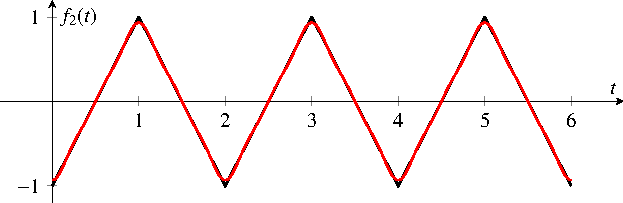
\includegraphics{papers/fourier/images/fourier_Dreieck.pdf}
	\caption{Fourierapproximation einer Dreieckfunktion}
	\label{fourier:fig:fourierdreieck}
\end{figure}

Im Beispiel zur Dreiecksfunktion (Abbildung~\ref{fourier:fig:fourierdreieck}) entspricht  
\begin{equation}
	f_1(t) = \sum_{\substack{n=1 \\ n\ \text{ungerade}}}^{5} \frac{-8}{\pi^2 n^2} \cos(n\pi t)
\end{equation}
der roten Kurve und überdeckt das Original nahezu perfekt und das mit nur drei Summanden.  
Da $f_1$ gerade ist, sind alle Sinuskoeffizienten $b_n=0$ und die Kosinuskoeffizienten bleiben nur für ungerade $n$ ungleich $0$.  
Der Mittelwert ist $a_0=0$.  
Bei der Fourier-Reihenbildung kann man sich viel Zeit ersparen, wenn man zuerst überprüft, ob es sich um eine gerade oder ungerade Funktion handelt.
So kann man ohne zu rechnen $a_n$ oder $b_n$ gleich Null setzen.
\end{beispiel}



\begin{beispiel}

%
% fig-strahlungsspektren.tex
%
% (c) 2025 Prof Dr Andreas Müller
%
\begin{figure}
	\centering
	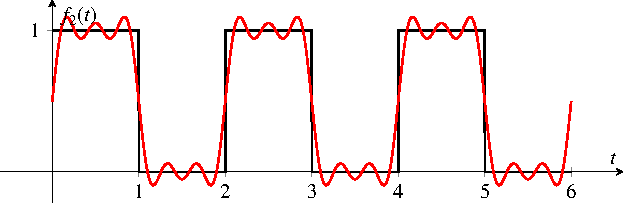
\includegraphics{papers/fourier/images/fourier_Rechteck.pdf}
	\caption{Fourierapproximation einer Rechteckfunktion, bei der in der Nähe der Sprungstellen das Gibbs-Phänomen auftritt.%
	\label{fourier:fig:fourierrechteck}}
\end{figure}

In der Rechtecksfunktion (Abbildung~\ref{fourier:fig:fourierrechteck}) mit Sprungstelle tritt das Gibbssche Phänomen auf.  
In der Nähe eines Sprungs entsteht ein charakteristischer Überschwinger, der selbst bei unendlich vielen Summanden nicht verschwindet.
Das Gleichheitszeichen in \eqref{eq:fourier} gilt daher nur eingeschränkt.  
Die Fourier-Reihe bis $n=5$ lautet
\begin{equation}
	f_2(t) = \frac{1}{2} + \sum_{\substack{n=1 \\ n\ \text{ungerade}}}^{5} \frac{2}{\pi n} \sin\left( \pi n t \right)
\end{equation}
und entspricht der roten Kurve.  
Da die Rechteckfunktion um den Mittelwert $\frac{a_0}{2}=\frac{1}{2}$ ungerade ist, sind alle Cosinuskoeffizienten $a_n=0$ und die Sinuskoeffizienten bleiben nur für ungerade $n$ ungleich $0$.  

\end{beispiel}






